\addtolength{\textheight}{-10pt}

\section{EXPERIMENTS}
\label{sec:experiments}

\subsection{Training}
To train our networks, we used the PyTorch\footnote{\url{https://github.com/pytorch/pytorch}} deep learning framework. The networks were trained using the Adadelta Optimizer \cite{DBLP:journals/corr/abs-1212-5701}.

The loss function used for training and validation was Mean Squared Error  (MSE) Loss. During the training phase, the loss was calculated across all values outputted by the network, i.e., across all ten time steps following the formula
\begin{equation} \label{eq:1}
MSE_{train} = \dfrac{1}{2n}(\sum_{t=1}^{n}(s'_t -  s_t)^2 +(m'_t - m_t)^2)
\end{equation}
where $n=10$ is the number of time steps in our case, $s_t$  and $m_t$ are the steering and motor values respectively outputted by the network at a given time step, and $s'_t$ and $m'_t$ are the expert steering and motor values at a given timestep.

During validation, a similar MSE loss metric was used except the loss was calculated only for the two final motor and steering output as given by
\begin{equation} \label{eq:2}
MSE_{validation} = \dfrac{1}{2}((s'_n -  s_n)^2 +(m'_n - m_n)^2)
\end{equation}
Only the final timestep was used in measuring the validation accuracy of the networks as this is the only value which is used for evaluation on the model vehicles, and thus the only value which affects the driving performance of the model car. We chose to use the MSE loss function, as small deviations from expert driving were considered normal while larger deviations are reflective of a problem in the network's control and thus have a greater effect on the calculated error. The quadratic error curve of MSE loss allows for such results and closely mimics results from the percentage autonomy metric introduced later in the paper in which small deviations have an inconsequential effect on performance.

The same set of training data were used for each of the networks, as well as the same unseen validation set. All experiments were replicated eight times with randomly initialized networks and shuffled datasets. The results here depict the mean across these trials, with error bars representing 95\% confidence intervals.

Our dataset contains approximately 1.93 million usable data moments for training and validation on the networks. 10\% of the collected data were kept for use in an unseen validation dataset for the evaluation of the networks. All data were equally distributed for each modality in both the training and validation sets. 

\begin{figure}[t]
\centering
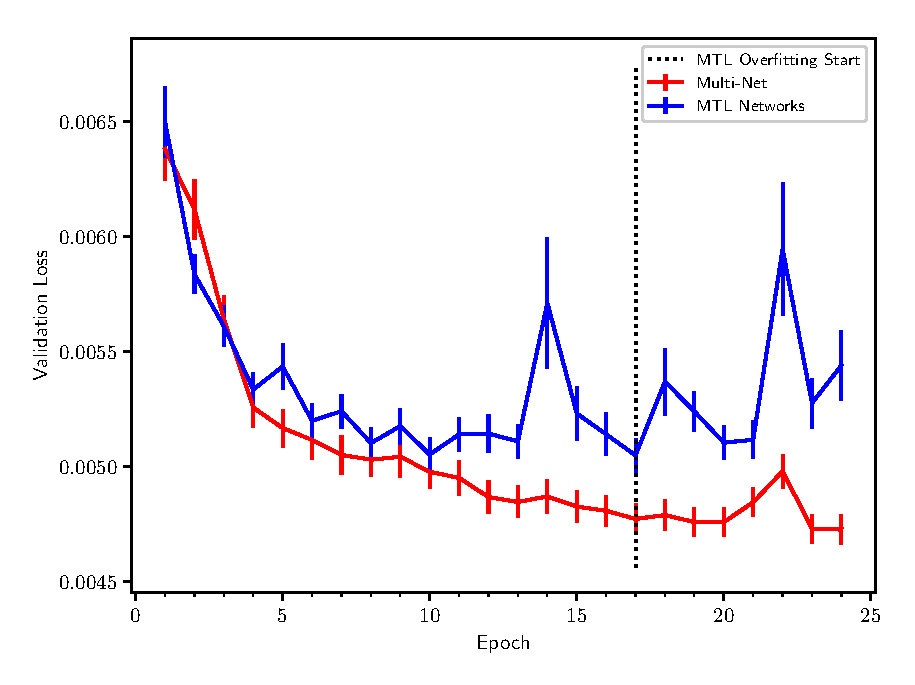
\includegraphics[width=\linewidth]{paper/content/images/mtl}
\caption{Multi-Modal Validation of MultiNet and MTL Networks with 95\% Confidence Intervals}
\label{fig:lve}
\end{figure}

\subsection{Multi-Modal Comparison}
\label{resultspt1}
In our initial experiment a MultiNet Z2Color network trained in a multi-modal dataset of direct, follow, and furtive was compared to three MTL Z2Color networks trained on direct, follow, and furtive modes separately. The networks were than evaluated using the validation loss measurement described in \Cref{eq:2}. The results are summarized in \Cref{fig:lve} where the losses of the three MTL networks are averaged across the modes for direct comparison to the MultiNet models.

Initially, from epochs 1 to 4, the MultiNets have similar but slightly poorer performance compared to the MTL networks. This is due to the wide variety of data the MultiNets receive requiring greater generalization initially, while the MTL networks can immediately specialize to specific modes.

From epochs 4 to 10, the MultiNets begin to surpass the MTL networks while remaining close in performance. During this period we hypothesize that the MTL networks begin to differentiate between individual driving modalities by using the provided modal information data.

From epochs 10 to 17, the MultiNets drastically outperform the MTL networks, which flatten off in their loss curve here. The MTL loss curve begins to move erratically by getting caught in various local minima. However it doesn't yet begin overfitting, which we characterize as consistently having a loss value above the absolute minimum. The MultiNets steadily improve through the use of the additional modal data. From epochs 17 to 24, the MTL networks begin to overfit dramatically, while the MultiNets continue to decline in loss despite a small bump at epochs 21 and 22. This suggests MTL networks are more susceptible to overfitting and local minima than their MultiNet counterpart. This is likely due to the variety of data the MultiNet networks are exposed to allowing for greater generalization across modes, while maintaining individual behavioral characteristics in specific modalities.

\begin{figure}[t]
\centering
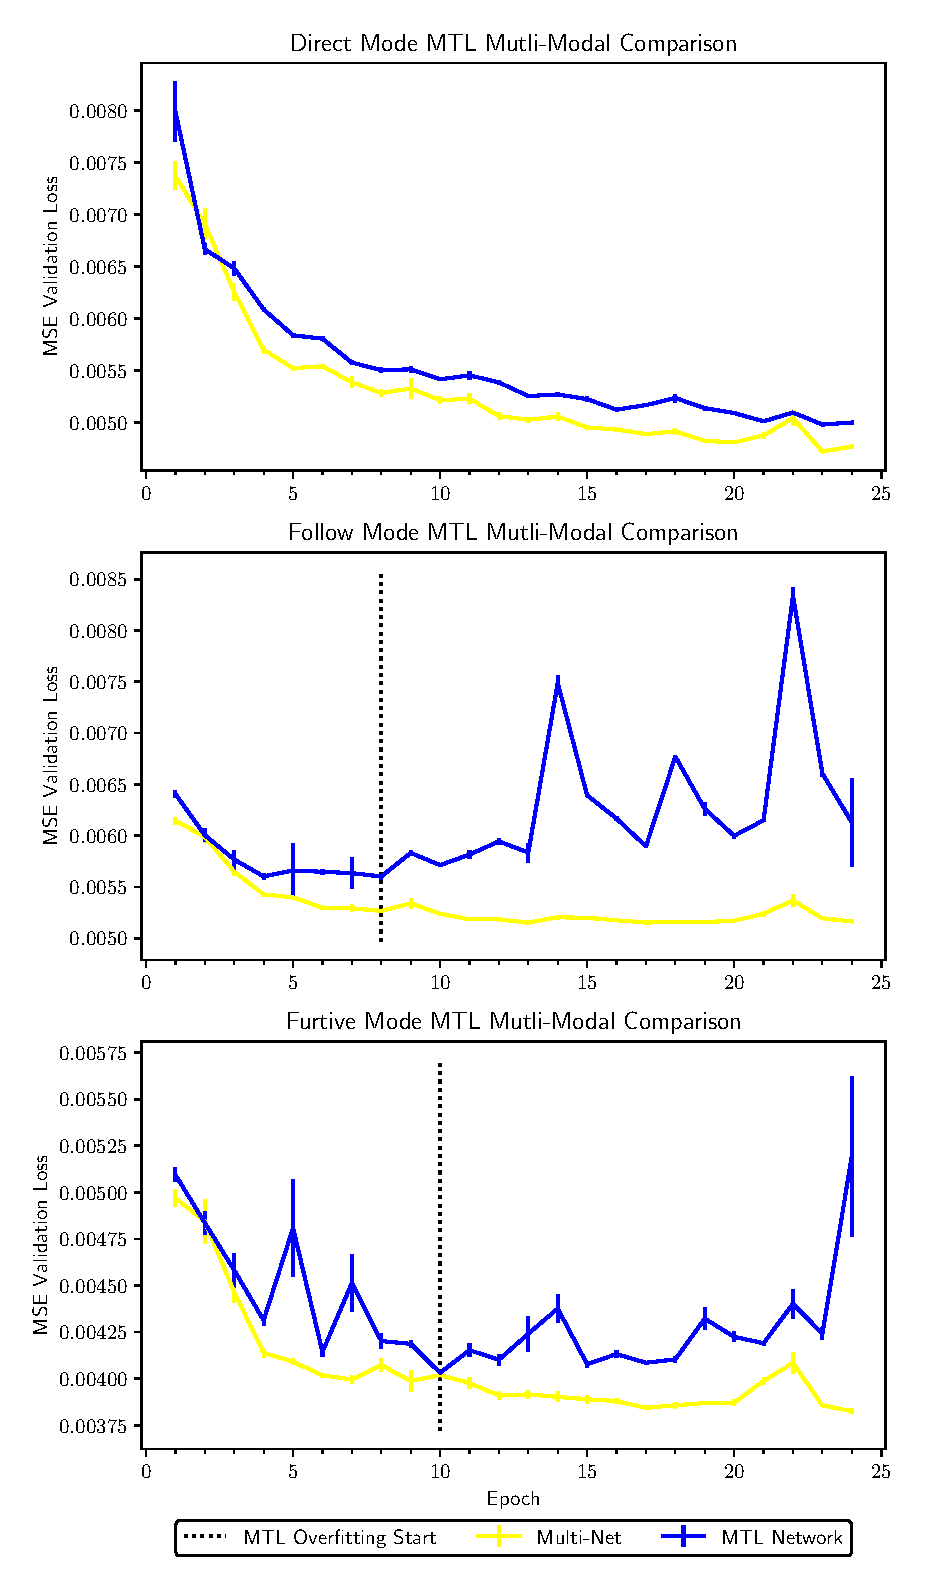
\includegraphics[width=\linewidth]{paper/content/images/individual_new}
\caption{Individual Validation of MultiNet and MTL Networks with 95\% Confidence Intervals in Direct, Follow, and Furtive Modes}

\label{fig:furtivegraph}
\end{figure}


\subsection{Performance in Individual Modes}
\label{resultspt2}
To further investigate the network's performance in individual behavioral modes, further experiments were done to compare the MultiNet models to a single MTL network in individual modes. These experiments were conducted to evaluate how the MultiNet displays behaviors distinct to the individual driving modes. In the experiments depicted in \Cref{fig:furtivegraph}, the MultiNet models were trained on Direct, Folow, and Furtive data in each experiment while the MTL networks were trained only on the data for that experiment, e.g., for the furtive graph the MTL network was trained and validated on furtive data. Validation was done only on the data for the appropriate mode of each network, i.e.\, both the MTL and MultiNet models were evaluated only in furtive mode for the furtive graph.

In the first mode, direct mode, it is clear that both networks have similar performance levels. In the second epoch, the MTL networks outperformed the MultiNet networks, this is likely due to initial confusion between the behavioral modalities in the MultiNet networks. After this point we hypothesize the MultiNet models learnt the modal distinctions and thus continued to have lower loss measurements than their MTL counterparts until the end of training. Both networks seemed to learn the direct mode task quickly and had no large fluctuations in loss or overfitting as compared to the graphs for each of the other modes. This suggests direct mode is the simplest task as it doesn't involve any special behavioral activity and simply involves avoiding obstacles in the vehicle's path. 

In follow mode, the MTL networks consistently had a higher validation loss than the MultiNet networks. In the second epoch both networks had a similar validation error, but after this point the networks quickly diverged. The MTL networks seemed to flatten out and stop learning significantly after the fourth epoch. By the eighth epoch the follow mode network begins to overfit and steadily increase in loss. Meanwhile, the MultiNet network continues to become more accurate throughout the training other than in two small bumps in the loss in the ninth and twenty-second epoch. These results suggest that MultiNet networks are more capable of learning complex tasks like following, while plain MTL networks are susceptible to overfitting and less capable of learning specific behaviors with the same number of parameters. The results also demonstrate the difference in complexity of the follow mode when compared to the simple direct modality.

In furtive mode, the initial performance in the first four epochs was the same as what was observed for direct and follow mode. It is clear that the multi-modal models seemed to require approximately two epochs of training to begin to distinguish between different modes and develop distinct behaviors. Starting from the fifth epoch, the MTL networks began to oscillate rapidly in the recorded validation loss. This suggests that the MTL networks had found their minima already and were thus oscillating in this region. After the tenth epoch, the MTL models reached their minimum average validation loss. The MultiNet models continued to learn throughout the training period, achieving the lowest validation error at the end of the twenty-four epochs. This suggests the propensity of the MultiNet networks for continuous learning without overfitting as well as for performing in complex behavioral modes like furtive mode.

% Please add the following required packages to your document preamble:
% \usepackage{booktabs}
\begin{table}[]
\begin{center}
\begin{tabular}{l|l|l|}
\cline{2-3}
                                                         & \multicolumn{2}{l|}{\textbf{EVALUATION MODE}} \\ \hline
\multicolumn{1}{|l|}{\textbf{NETWORK}}                   & \textit{Direct}       & \textit{Furtive}      \\ \hline
\multicolumn{1}{|l|}{\textit{MultiNet}}                  & 92.68\%               & 88.23\%               \\ \hline
\multicolumn{1}{|l|}{\textit{MTL}}                       & 84.27\%               & 87.55\%               \\ \hline
\multicolumn{1}{|l|}{\textbf{$\Delta$ (MultiNet - MTL)}} & 8.31\%                & 0.68\%                \\ \hline\hline
\multicolumn{1}{|l|}{\textbf{$\Delta$ Validation Loss \%}} & 8.16\%                & 12.58\%                \\ \hline
\end{tabular}
\end{center}
\caption{Percentage Autonomy and $\Delta$ Validation Loss \% in Direct and Furtive Modes}
\label{resultsauto}
\end{table}

\subsection{Evaluation on Model Cars}

To test the proficiency of the models in real world driving situations, we measure the percentage autonomy metric \cite{bojarski2016end} measured as

\begin{equation}
    autonomy = (1 - \dfrac{correction\ time}{elapsed\ time}) \cdot 100
   \label{eq:autonomy}
\end{equation}

For the live experiments, both MTL and MultiNet networks were evaluated on a winding 200 m loop of sidewalk (\Cref{fig:evalpath}) with sufficient obstacles within a one hour interval. Only direct and furtive modes were used when evaluating the cars, while follow mode was excluded because t he driving of the leader car may differ between runs making a quantitative analysis impractical. The networks for on the road evaluation were chosen at the point of minimum average validation error across the trials, i.e., we chose the epoch and trial which minimized the average validation error for both the MultiNet and MTL networks. This minimum occured at epoch 23 on a specific trial, before either network began to overfit. 


The results from our live experiments are depicted in \Cref{resultsauto}. It is apparent that the MultiNet networks were superior to the MTL networks in both evaluation modes. However the difference is more pronounced in the direct mode than the furtive mode. To understand why this is occurring, we have to take a careful look at the autonomy metric which is used to measure performance.

The standard autonomy metric is a good indicator of performance in direct mode, as performance in this mode is solely based on the network's path following and obstacle avoidance abilities. The autonomy metric directly measures this ability.
The furtive mode on the other hand, involves more complex driving behaviors such as speed modulation near foliage, staying close to observed boundaries, in addition to path following and avoiding obstacles. The autonomy metric does not measure these subtle behaviors.
When driving near the edge the chance of going off course is greater and hence the vehicle requires more manual correction. This effectively reduces the autonomy measurement. For these reasons, the standard autonomy metric isn't sufficient when measuring performance in a furtive driving mode in which more complex behaviors than obstacle avoidance are involved.

When observing the MTL and MultiNet networks qualitatively in furtive mode, it is clear that the MultiNet network exhibits more pronounced furtive speed modulation behavior while staying close to boundaries when compared to the MTL network. This characteristic furtive behavior demonstrates the ability of MultiNet networks to act distinctly in multiple behavioral modes with the use of inserted modal data. We have included a supplementary AVI format video which contains segments of footage from each of the live experiments as well as examples of each driving mode. This will be available at \url{http://ieeexplore.ieee.org}.

\subsection{Results Verification}
To verify the results from the validation metric in \Cref{resultspt1} and \Cref{resultspt2}, we computed the percentage difference in performance according to the validation loss to compare the MSE loss metric to the autonomy metric in the live experiments. The percentage difference in validation loss was computed with the following equation:

\begin{equation}
\Delta\ Loss\ \% = \dfrac{MTL\ Loss - MultiNet\ Loss}{MultiNet\ Loss} \times 100
\end{equation}

The $\Delta \ Loss$ \% values for MultiNet and MTL networks in both Direct and Furtive mode are displayed at the bottom of \Cref{resultsauto}. For direct mode, the $\Delta \ Loss$ \% is very similar to the percentage difference in autonomy. This suggests the MSE loss metric is a valid indicator for a network's driving performance. For the furtive mode, the $\Delta \ Loss$ \% is significantly greater than the difference in autonomy which suggests the MSE loss metric used for validation effectively accounts for a network's display of characteristic behaviors in a behavioral mode which were observed qualitatively. This supports the conclusions made earlier from analysis of MultiNet and MTL performance using the MSE loss metric.
